\documentclass[12pt,letterpaper]{article}
\usepackage{amsmath,amsthm,amsfonts,amssymb,amscd}
\usepackage{listings}
\usepackage{color}
\usepackage{MnSymbol,wasysym}
\usepackage{caption}
\usepackage{subcaption}
\definecolor{codegreen}{rgb}{0,0.6,0}
\definecolor{codegray}{rgb}{0.5,0.5,0.5}
\definecolor{codepurple}{rgb}{0.58,0,0.82}
\definecolor{backcolour}{rgb}{0.95,0.95,0.92}
\definecolor{dkgreen}{rgb}{0,0.6,0}
\definecolor{gray}{rgb}{0.5,0.5,0.5}
\definecolor{mauve}{rgb}{0.58,0,0.82}

\usepackage{biblatex}

\addbibresource{bibliography.bib}

\lstdefinestyle{mystyle}{
  language=R,
  backgroundcolor=\color{backcolour},   commentstyle=\color{codegreen},
  aboveskip=3mm,
  belowskip=3mm,
  showstringspaces=false,
  columns=flexible,
  basicstyle={\small\ttfamily},
  numbers=left,
  numbersep=5pt,
  numberstyle=\tiny\color{gray},
  keywordstyle=\color{blue},
  commentstyle=\color{dkgreen},
  stringstyle=\color{mauve},
  breaklines=true,
  breakatwhitespace=true
  tabsize=3
}

\lstset{style=mystyle}
\usepackage{hyperref}
\usepackage{graphicx}
\usepackage{enumerate}
\usepackage{fancyhdr}
\usepackage{mathrsfs}
\usepackage[margin=3cm]{geometry}
\setlength{\parindent}{0.0in}
\setlength{\parskip}{0.05in}

% Edit these as appropriate
\newcommand\course{CS432}
\newcommand\semester{Spring 2016}     
\newcommand\hwnum{6}
\newcommand\yourname{Kevin R. Clemmons}
\newcommand\login{oduprogrammer16}

\newenvironment{answer}[1]{
  \subsubsection*{Problem #1}
}

\pagestyle{fancyplain}
\headheight 40pt
\lhead{\yourname\ \\(\login)\\\course\ --- \semester}
\chead{\textbf{\Large Assignment \hwnum}}
\rhead{\today}
\headsep 40pt

\begin{document}

All files mentioned in this file are uploaded into the {\it github} repository.

The \LaTeX code invovled in the generation of this document was aided by the example code provided in the links that Dr. Nelson sent out on January 17, 2016\cite{mohammedaturban2013}. 

This document was compiled on \url{www.sharelatex.com}

\begin{answer}{1}
Before starting to work on the D3 Graph, a script was written to extract the data from my twitter account. 

First a list of all of my followers was created and written to a text file called {\it kevinfollowers.txt}. This file is primarily used for backup. Then the program goes through the list of all of my followers and for each follower, checks the other followers to determine if the follower follows the other followers. The function that determines if a person follows another person is found the tweepy library\cite{joshuarosslein2009}. This code is found in Listing 1 and the final result is a csv file which describes a list of edges in the format (follower,personFollowing). In addition, this program utilizes a credential library that I developed, to  manage my twitter authorization credentials. The code for this credential library is located at my repository via the following link \url{https://github.com/oduprogrammer16/CredentialManager}.
 
 \begin{lstlisting}[langauge=Python,caption=Determining if a follower follows another follower]
 try:
	result = api.show_friendship(source_screen_name=user,target_screen_name=follower)
	
except tweepy.RateLimitError:
	printEdgeList(edgeList,'kevin_network.csv')
	printEdgeList(unknownEdges,'unknownEdges.csv')
	print("\t\tRate Limit Error Exceeded: sleeping for 15 minutes")
	time.sleep(15 * 60)
	result = api.show_friendship(source_screen_name=user,
	target_screen_name=follower)

except tweepy.TweepError as e:
	pass

if result is not None:
	if result[1].following:
		edgeList.append((follower,user))
else:
	unknownEdges.append((follower,user))
 \end{lstlisting}
\newpage 
It should be noted that this code is not effecient. A better strategy for determining who follows who in my follower list would be to get a follower's screen-name and then determine who they follow in my follower list. 

The code that was ran to extract the followers and who they follow in my follower list took exactly 4 hours, 29 minutes and thirty one seconds. This due to the fact that the twitter api only allows 180 requests every 15 minutes. \cite{twitterinc2016}

After the data was extracted, a visual graph was created using D3\cite{mikebostock2015}. The graph was created in an html file called {\it followergraph.html} and the is a modified version of Mike Bostock's basic directional force layout diagram\cite{mikebostock2016}. Figure 1 shows my network graph. This graph can also be viewed via the following url: \url{http://www.cs.odu.edu/~kclemmon/follower_graph.html}
 
\begin{figure}[ht!]
\centering 
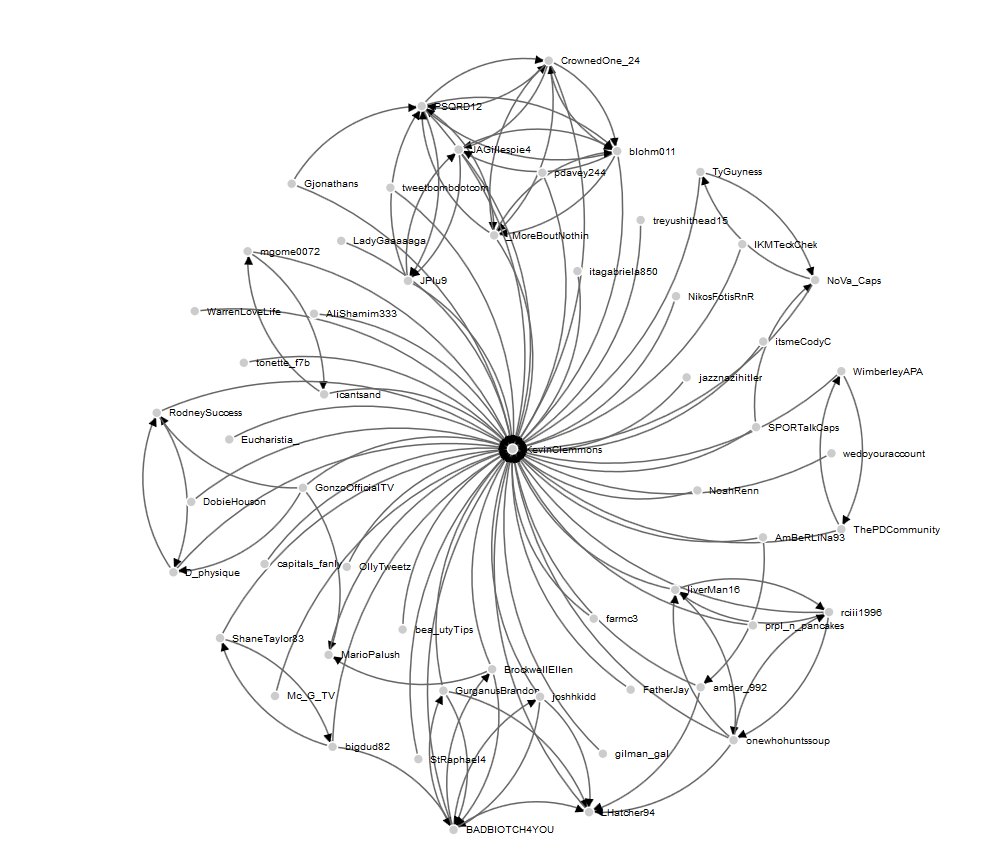
\includegraphics[scale=0.55]{FollowerGraph}
\caption{Follower Network}
\label{overflow}
\end{figure}
\newpage 

\end{answer}
To determine Gender Homophily, a list of followers  and their names was obtained from my twitter account using the twitter api\cite{joshuarosslein2009}. Once all the names were obtained, the genders of each follower was estimated using the the gender-detector library\cite{marcosvanetta2014}. The genders for all the followers are dumped into a json file called {\it backup2.json}. The program was able to obtain genders for 29 followers and was unable to obtain genders for 27 followers. Table 1 lists the users in which a gender was successfully estimated and Table 2 lists the users in which a gender was not successfully estimated. 


\newpage 
\begin{table}[ht!]
    \centering
    \begin{tabular}{|c|c|c|}\hline
    \textbf{Username} & \textbf{Name} & \textbf{Gender} \\\hline
    JPlu9 & Jared Pluciniczak & male \\ \hline 
    StRaphael4 & St Raphael & male \\ \hline 
    joshhkidd & Joshua Reynolds  & male \\ \hline 
    Dphysique & Dynasty For Life Rec & female \\ \hline 
    beautyTips & Beauty Tips  & female \\ \hline 
    JAGillespie4 & Justin Gillespie & male \\ \hline 
    Gjonathans & Jonathan Gustafsson & male \\ \hline 
    MarioPalush & MARIO & male \\ \hline 
    LadyGaaaaaga & Lady Gaga & female \\ \hline 
    GurganusBrandon & Brandon Gurganus & male \\ \hline 
    amber992 & Amber Schakel & female \\ \hline 
    KevinClemmons & Kevin Clemmons & male \\ \hline 
    NoahRenn & Noah Renn & male \\\hline 
    rciii1996 & Robert RCIII Croson & male \\\hline 
    CrownedOne24 & Steven & male \\\hline 
    itagabriela850 & gabriela & female \\\hline 
    treyushithead15 & trey peters & male \\\hline 
    bigdud82 & Mike Dudley & male \\\hline 
    RodneySuccess & Rodney Pickett II & male \\\hline 
    ThePDCommunity & Kevin McCarthy & male \\\hline 
    PSQRD12 & Paul Porter & male \\\hline 
    AliShamim333 & Shamim & female \\\hline 
    LHatcher94 & luke & male \\\hline 
    liverMan16 & Eric Liverman & male \\\hline 
    AmBeRLiNa93 & Amber Schakel & female \\\hline 
    WarrenLoveLife & Warren Happy â & male \\\hline 
    prplnpancakes & Daniel Pancake & male \\\hline 
    BrockwellEllen & Ellen brockwell & female \\\hline 
    DobieHouson & dobie houson & male \\\hline 
    \end{tabular}
    \caption{Followers that a Gender was Obtained}
    \label{tab:my_label}
\end{table}
\begin{table}[ht!]
    \centering
    \begin{tabular}{|c|c|}\hline
    \textbf{Username} & \textbf{Name}  \\\hline
    jazznazihitler & jay z\\\hline 
    WimberleyAPA & Wimberley APA (WAPA)\\\hline 
    tweetbombdotcom & TweetBomb.com\\\hline 
    tonettef7b & tonettef7b\\\hline 
    pdavey244 & Pat\\\hline 
    McGTV & Mc G TV\\\hline 
    NoVaCaps & NoVa Caps\\\hline 
    IKMTeckChek & IKM TeckChek\\\hline 
    BADBIOTCH4YOU & .\\\hline 
    SPORTalkCaps & Capitals SPORTalk\\\hline 
    blohm011 & Hunter Blohm\\\hline 
    capitalsfanly & Capitals Report\\\hline 
    gilmangal & cabbage patch kid\\\hline 
    GonzoOfficialTV & GONZO\\\hline 
    ShaneTaylor83 & Shane Taylor\\\hline 
    onewhohuntssoup & Hunter Zupo\\\hline 
    TyGuyness & Tyler Humphries\\\hline 
    wedoyouraccount & wedoyouraccounting\\\hline 
    OllyTweetz & I Follow Back ;) !\\\hline 
    NikosFotisRnR & NikosFotisR'nRoller\\\hline 
    farmc3 & A. P. Parsley\\\hline 
    MoreBoutNothin & Scott, Marquis\\\hline 
    FatherJay & Jay Wagner\\\hline 
    mgome0072 & mg\\\hline 
    icantsand & Sandy 'man' Wilson\\\hline 
    Eucharistia & Real Presence\\\hline 
    itsmeCodyC & Cody Crampton\\\hline 
    \end{tabular}
    \caption{Followers that a Gender was not Obtained}
    \label{tab:my_label}
\end{table}
\newpage 

Once The genders were obtained, a new csv file called {\it kevinGenderNetwork} was generated and contains a reduced number of edges. This is due to the fact that the edges who had nodes in which a gender was deemed unknown were eliminated from the graph. Figure 2 shows the network without the nodes in which a gender could not be obtained. This graph can also be viewed via the following link \url{http://www.cs.odu.edu/~kclemmon/gender_graph.html}.
\newpage 
\begin{figure}[ht!]
\centering 
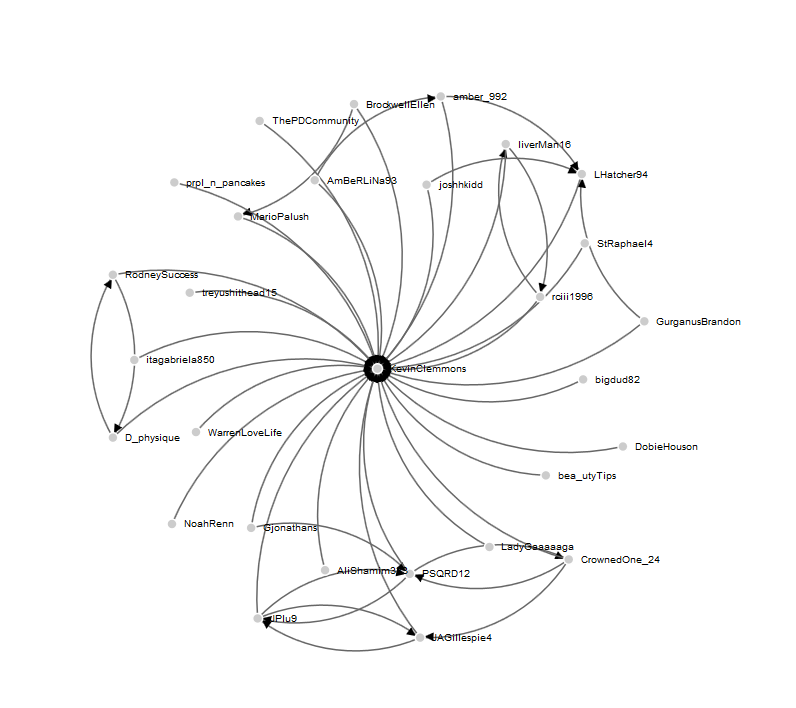
\includegraphics[scale=0.55]{genderGraph}
\caption{Gender Network}
\label{overflow}
\end{figure}

To compute the gender homophlly of the graph, let $p$ be the ratio of male to male edges to the total number of edges, $q$ be the ratio of female to female edges to the total number of edges and $r$ represent be the ratio of cross gender edges to the total number of edges. Gender homophilly of the graph exists if $r < 2pq$\cite{michaelnelson}. 

To compute $p,q$ and $r$, A program called {\it genderHomophily.py} iterates through the edges, and computes $p,q,r$ and $2pq$ The counts are then divided by the total number of edges. \\ \\ The following results were obtained below: 
\begin{itemize}
    \item $p = 0.02$ 
    \item $q = 0.71$
    \item $r = 0.26$
    \item $2pq = 0.031$
\end{itemize}
\newpage 
Since $r > 2pq$, gender homophily exists for my graph. 
\printbibliography
\end{document}
